\documentclass{llncs}
\usepackage{amsmath,amssymb}
\usepackage{tikz}
\usetikzlibrary{matrix,chains,scopes}

\title{Abstractions for Symbolic Sets}

\author{Arlen Cox, Xavier Rival}

\institute{Inria/CNRS/ENS Paris}

\begin{document}
    
\maketitle
% single abstract state
\renewcommand{\abstract}{\Sigma}
% set of all abstract states
\newcommand{\abstracts}{\textsc{AbsStates}}
% cardinality of a set
\newcommand{\card}[1]{|{#1}|}
% complement of a set
\newcommand{\comp}[1]{{#1}^{\mathrm{c}}}
% individual set variables: W, X, Y, or Z
% set of all set variables
\newcommand{\setvars}{\textsc{SetVars}}
% concrete state
\newcommand{\state}{\sigma}
% set of all concrete states
\newcommand{\states}{\textsc{States}}
% set of all values
\newcommand{\values}{\textsc{Vals}}
% concrete set c
% syntax of a logical constraint L
% syntax of a set expression E
% power set of a set
\newcommand{\powerset}[1]{\mathcal{P}\left({#1}\right)}


\newcommand{\defeq}{\stackrel{\textrm{\tiny def}}{=}}

%1. Introduction (1.5 pages)
%- Goals:
%- Set abstractions serve a different purpose than SAT/SMT/MC
%- Inference vs Entailment
%- Explicit vs Implicit control flow
%- Handling of quantifiers
%- Forward vs backward analysis
%- Modern set abstractions offer performance and precision
%- Set abstractions are useful for a wide variety of problems
%
%2. Overview (2 pages)
%-> a couple of examples, showing very intuitively (possibly just with pictures)
%the need for set abstractions
%Possibly:
%- a quick picture of HOO
%- a quick picture of Huisong's work
\input{overview.tex}


%3. Set Abstraction Problem (1 page)
%-> set up problem framework / why abstract domain vs other things?
%- Boolean Algebra
%- Cardinality/Value considerations
%- Forward analysis to be use as a subcomponent of other analyses
%- Abstract domain (implicit vs explicit control flow)
%- Inference (vs BAPA)
%
%4 Constructed set abstractions (5 pages)
%-> search for efficient structures and algorithms associated to them
%4.1 Lin
%4.2 QUICr
%4.3 BDD
%4.4 EQ functor
%4.5 Packing functor
%- Why packing doesn't work for BDDs in model checking, but does work here.
%
%5. Solver-based set abstractions (1.5 pages)
%-> encode problem to traditional, known problem
%5.1 SMT
%5.2 QBF
%
%
%6. Evaluation (2 pages)
%-> compare approaches in several classes of problems
%- Benchmark suites:
%- Python set tests
%- JSAna JavaScript verification
%- Memcad C data structure memory safety
%- Show:
%- Old set domains much slower
%- New set domains faster and often more precise
%- SMT doesn't scale in on these applications
%
%7. Tradeoffs/Limitations (0.5 pages)
%-> limitations and possible enhancements
%- Cardinality
%- Contents
%
%8. Related Work (1 page)
%
%9. Conclusions (0.5 pages)
    
    
    
\section{Logic and Set Abstraction}
\label{sec:logic-and-set-abstraction}

In this section we present the logical underpinnings of our class of set abstractions.  We are interested in a subclass of sets where sets are purely symbolic.  A \emph{purely symbolic set abstraction} is an abstraction for sets that places no requirements on the type or capabilities of the values stored within the set.  It does this by not allowing the expression of values within the logic.

In this paper, we use symbols $W$, $X$, $Y$, and $Z$ to represent set variables in $\setvars$.  We use $\state$ to represent a concrete state in $\states$ and we use $\abstract$ to represent an abstract state in $\abstracts$.
\begin{definition}[Symbolic Sets]
    Symbolic sets are defined by the following grammar:
    
    \begin{align*}
        L ::= & \ L \wedge L \ | \ E \subseteq E \ | \ \card{X} = 1 \ | \ \top \ | \ \bot &
        E ::= & \ \emptyset \ | \ X \ | \ \comp{E} \ | \ E \cup E
    \end{align*}
\end{definition}

A symbolic set consists of basic set combination operations with equality, non-strict subset and simple cardinality.  While more general symbolic sets can reasoned about by extending the cardinality (as in BAPA), the goal here is to perform invariant generation, so the problem goes beyond that of deciding implication.  We must also approximate upper bound operations.  As a result, the logic is simplified in such a way that is simultaneously useful and more amenable to computing upper bounds.

Symbolic sets represent concrete set states.  A concrete set state maps set variables to sets of values:
\begin{align*}
    \state \in \states = \setvars \rightarrow \powerset{\values}
\end{align*}

The meaning of these contraints is straightforward, but we give a formal definition for clarity.  A model of a set expression $E$ is a concrete state $\state$ and a set of concrete values $c$.  A model of a logical expression $L$ is a concrete state $\state$.  The concretization is given in terms of the models relationship.
\begin{align*}
  & \state, c \models \emptyset \textrm{ iff } c = \emptyset \qquad \state, c \models X \textrm{ iff } c = \state(X) \\
  & \state, c \models \comp{E} \textrm{ iff } \state, c' \models{E} \textrm{ and } \forall v \in \values. \; v \in c \leftrightarrow v \not\in c' \\
  & \state, c \models E_1 \cup E_2 \textrm{ iff } \state, c_1 \models E_1 \textrm{ and } \state, c_2 \models E_2\\
  & \qquad \qquad \qquad \qquad \qquad  \textrm{ and } \forall v \in \values. \; v \in c \leftrightarrow v \in c_1 \vee v \in c_2 \\
  & \state \models L_1 \wedge L_2 \textrm{ iff } \state \models L_1 \textrm{ and } \state \models L_2 \qquad \state \models \top \qquad \state \not\models \bot \\
  & \state \models E_1 \subseteq E_2 \textrm{ iff } \state, c_1 \models E_1 \textrm{ and } \state, c_2 \models E_2 \textrm{ and } \forall v \in \values. \; v \in c_1 \rightarrow v \in c_2 \\
  & \state \models \card{E} = 1 \textrm{ iff } \state, c \models E \textrm{ and } \exists v \in \values. \; c = \{v\} \\
  & \gamma(L) = \{\ \sigma \ |\  \sigma \models L\ \}
\end{align*}

We will also use the following derived logical forms for simplicity.
\begin{align*}
 & E_1 = E_2 \defeq E_1 \subseteq E_2 \wedge E_2 \subseteq E_1 \\
 & E_1 \cap E_2 \defeq \comp{(\comp{E_1} \cup \comp{E_2})} \\
 & E_1 \setminus E_2 \defeq E_1 \cap \comp{E_2} \\
 & E_1 \uplus E_2 \defeq E_1 \cup E_2 \textrm{ if } E_1 \cap E_2 = \emptyset
\end{align*}

\subsection{Relationship with model checking}

Because set abstractions are closely related to Boolean algebras, it might be natural to wonder how set abstractions are related to hardware model checking.  There are existing fast algorithms for hardware model checking and the problem has been thoroughly studied.

The key differentiator between most abstract interpretation and model checking techniques is that model checking techniques are designed to be property directed.  A \emph{property directed} approach uses a known property that is trying to be proven as an input to invariant generation.  As a result, invariants that are generated are perhaps only suitable to prove that particular property (and weaker properties).  While abstract interpretation can be property directed, often it is not.  The purpose of abstract interpretation is to discover a superset of program behaviors and use those behaviors to prove many properties of programs.  Thus the goal of a property directed technique is different to that of most abstract interpreters.

Furthermore, the libraries that we describe in this paper are designed to be used in an externally defined abstract interpretation (Figure~\ref{fig:domain-usage}).  As a result, they are not designed to have full knowledge of the overall analysis.  They are instead designed to reason about set constraints describing a single abstract state.  The understanding of the analysis is relegated to the external entity that performs the abstract interpretation.  In other words, a set abstraction is to an abstract interpreter what a sat solver is to a hardware model checker.  The set abstractions are different from SAT solvers because they are designed to solve the kinds of problems that arise in abstract interpretation.

\begin{figure}[tb]
    \centering
    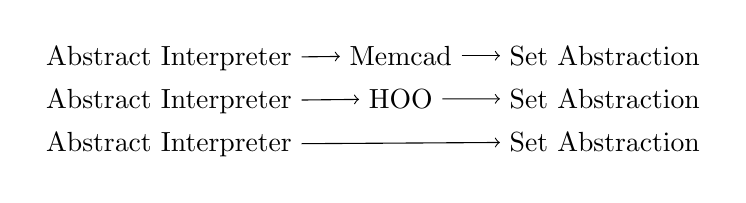
\begin{tikzpicture}[
    every on chain/.append style={join},
    every join/.style={->}
    ]
    \matrix (m) [matrix of nodes, column sep=5mm, nodes={}]
    {
        Abstract Interpreter & Memcad & Set Abstraction \\
        Abstract Interpreter & HOO & Set Abstraction \\
        Abstract Interpreter &     & Set Abstraction \\
    };
    { [start chain]
        \chainin (m-1-1);
        \chainin (m-1-2);
        \chainin (m-1-3);
    }
    { [start chain]
        \chainin (m-2-1);
        \chainin (m-2-2);
        \chainin (m-2-3);
    }
    { [start chain]
        \chainin (m-3-1);
        \chainin (m-3-3);
    }
    \end{tikzpicture}
    \caption{A set abstraction is used as part a larger analysis.  The abstract interpreter delegates some tasks to abstract domains.  Here, we consider three cases (1) Memcad is an abstract domain for C heaps that delegates some problems to a set abstraction; (2) HOO is an abstract domain for JavaScript heaps that delegates many problems to a set abstraction; and (3) The set abstraction is used directly}
    \label{fig:domain-usage}
\end{figure}

\paragraph{Key challenges:}  As opposed to model checkers, there are three additional challenges that a symbolic set abstraction faces. (1) Forward analysis of assignment introduces existential quantifiers.  They must be eliminated or otherwise handled by the abstraction.  The nesting of these quantifiers can be very deep. (2) The constraints are equality heavy and disjointness heavy.  Many constraints are simple equality ($X = Y$) or disjointness ($X \cap Y = \emptyset$).  (3) There are often many variables with few constraints on them.  Many variables may be introduced without being significantly constrained.

\paragraph{Key reliefs:}  As opposed to model checkers, symbolic set abstraction is easier in () ways. (1) There are often fewer variables.  Since not all variables are set variables, the total number of variables is significantly lower.  (2) Relationships between variables are not as complex.  Because the transition relation does not have to be included in the Boolean formulas, the set abstraction is only responsible for relationships that form between set variables.  These can be much simpler than what the full transition relation would dictate.  (3) Variables are often clustered into small groups that are tightly inter-related.  This means that packing and slicing techniques can be extremely beneficial.
    
\end{document}